\documentclass[%
  crop,%
  tikz,%
  multi=false%
]{standalone}%
\usepackage[utf8]{luainputenc}%
\usepackage[no-math]{fontspec}%
\defaultfontfeatures{%
  Numbers={OldStyle,Proportional},%
  Ligatures=TeX,%
  Extension=.ttf,%
}%
\setmainfont[%
  UprightFont=*-Regular,%
  ItalicFont=*-Italic,%
  BoldFont=*-Bold,%
  BoldItalicFont=*-BoldItalic,%
]{Raleway}%
\setsansfont[%
  UprightFont=*-Regular,%
  ItalicFont=*-Italic,%
  BoldFont=*-Bold,%
  BoldItalicFont=*-BoldItalic,%
]{Raleway}%
\usepackage[frenchmath]{mathastext}%
\usepackage{amsmath}%
\usepackage{amssymb}%
\usepackage{mathrsfs}%
\usepackage{mathtools}%
\usepackage{siunitx}%
\usepackage[siunitx]{circuitikz}%
\usetikzlibrary{calc,backgrounds,arrows.meta,patterns,positioning}%
\ctikzset{bipoles/length=1.2cm}%

% Colors
\usepackage{xcolor}%
\definecolor{RoseauGreen}{HTML}{cad40e}%
\definecolor{RoseauGrey}{HTML}{adb9cb}%
\definecolor{RoseauBlue}{HTML}{234e83}%

\DeclareMathOperator{\sign}{sign}%

% Sets
\let\C\relax
\newcommand{\R}{\ensuremath{\mathbb{R}}} % Real
\newcommand{\N}{\ensuremath{\mathbb{N}}} % Natural
% \newcommand{\C}{\ensuremath{\mathbb{C}}} % Complexes
\newcommand{\B}{\ensuremath{\mathscr{B}}} % Electrical buses
\newcommand{\Ch}{\ensuremath{\mathscr{C}}} % Loads
\renewcommand{\L}{\ensuremath{\mathscr{L}}} % Lines
\renewcommand{\P}{\ensuremath{\mathscr{P}}} % Phases

% Phases
\newcommand{\arm}{\ensuremath{\mathrm{a}}}%
\newcommand{\brm}{\ensuremath{\mathrm{b}}}%
\newcommand{\crm}{\ensuremath{\mathrm{c}}}%
\newcommand{\nrm}{\ensuremath{\mathrm{n}}}%
\newcommand{\grm}{\ensuremath{\mathrm{g}}}%
\newcommand{\abrm}{\ensuremath{\mathrm{ab}}}%
\newcommand{\bcrm}{\ensuremath{\mathrm{bc}}}%
\newcommand{\carm}{\ensuremath{\mathrm{ca}}}%
\newcommand{\anrm}{\ensuremath{\mathrm{an}}}%
\newcommand{\bnrm}{\ensuremath{\mathrm{bn}}}%
\newcommand{\cnrm}{\ensuremath{\mathrm{cn}}}%
\newcommand{\agrm}{\ensuremath{\mathrm{ag}}}%
\newcommand{\bgrm}{\ensuremath{\mathrm{bg}}}%
\newcommand{\cgrm}{\ensuremath{\mathrm{cg}}}%
\newcommand{\ngrm}{\ensuremath{\mathrm{ng}}}%
\newcommand{\abcrm}{\ensuremath{\mathrm{abc}}}%
\newcommand{\abcnrm}{\ensuremath{\mathrm{abcn}}}%

% Transformer
\newcommand{\Xrm}{\ensuremath{\mathrm{X}}}%
\newcommand{\Yrm}{\ensuremath{\mathrm{Y}}}%
\newcommand{\Zrm}{\ensuremath{\mathrm{Z}}}%
\newcommand{\xrm}{\ensuremath{\mathrm{x}}}%
\newcommand{\yrm}{\ensuremath{\mathrm{y}}}%
\newcommand{\zrm}{\ensuremath{\mathrm{z}}}%
\newcommand{\Arm}{\ensuremath{\mathrm{A}}}%
\newcommand{\Brm}{\ensuremath{\mathrm{B}}}%
\newcommand{\Crm}{\ensuremath{\mathrm{C}}}%
\newcommand{\Nrm}{\ensuremath{\mathrm{N}}}%

% Indices or exponents
\newcommand{\cons}{\ensuremath{\mathrm{cons.}}}%
\renewcommand{\prod}{\ensuremath{\mathrm{prod.}}}%
\newcommand{\theo}{\ensuremath{\mathrm{th.}}}%
\newcommand{\const}{\ensuremath{\mathrm{const.}}}%

% Variables
\newcommand{\umax}{\ensuremath{U^{\max}}}%
\newcommand{\umaxnorm}{\ensuremath{U^{\max\,\text{norm.}}}}%
\newcommand{\umin}{\ensuremath{U^{\min}}}%
\newcommand{\uminnorm}{\ensuremath{U^{\min\,\text{norm.}}}}%
\newcommand{\unom}{\ensuremath{U^{\text{nom.}}}}%
\newcommand{\unomnorm}{\ensuremath{U^{\text{nom.}\,\text{norm.}}}}%
\newcommand{\uup}{\ensuremath{U^{\text{up}}}}%
\newcommand{\uupnorm}{\ensuremath{U^{\text{up}\,\text{norm.}}}}%
\newcommand{\uupprime}{\ensuremath{U^{\text{up}\,\prime}}}%
\newcommand{\udown}{\ensuremath{U^{\text{down}}}}%
\newcommand{\udownnorm}{\ensuremath{U^{\text{down}\,\text{norm.}}}}%
\newcommand{\udownprime}{\ensuremath{U^{\text{down}\,\prime}}}%
\newcommand{\smax}{\ensuremath{S^{\max}}}%
\newcommand{\pmax}{\ensuremath{P^{\max}}}%
\newcommand{\sproj}{\ensuremath{\underline{S^{\text{proj.}}}}}%
%

\begin{document}
\ctikzset{european, straight voltages, cute inductors}%
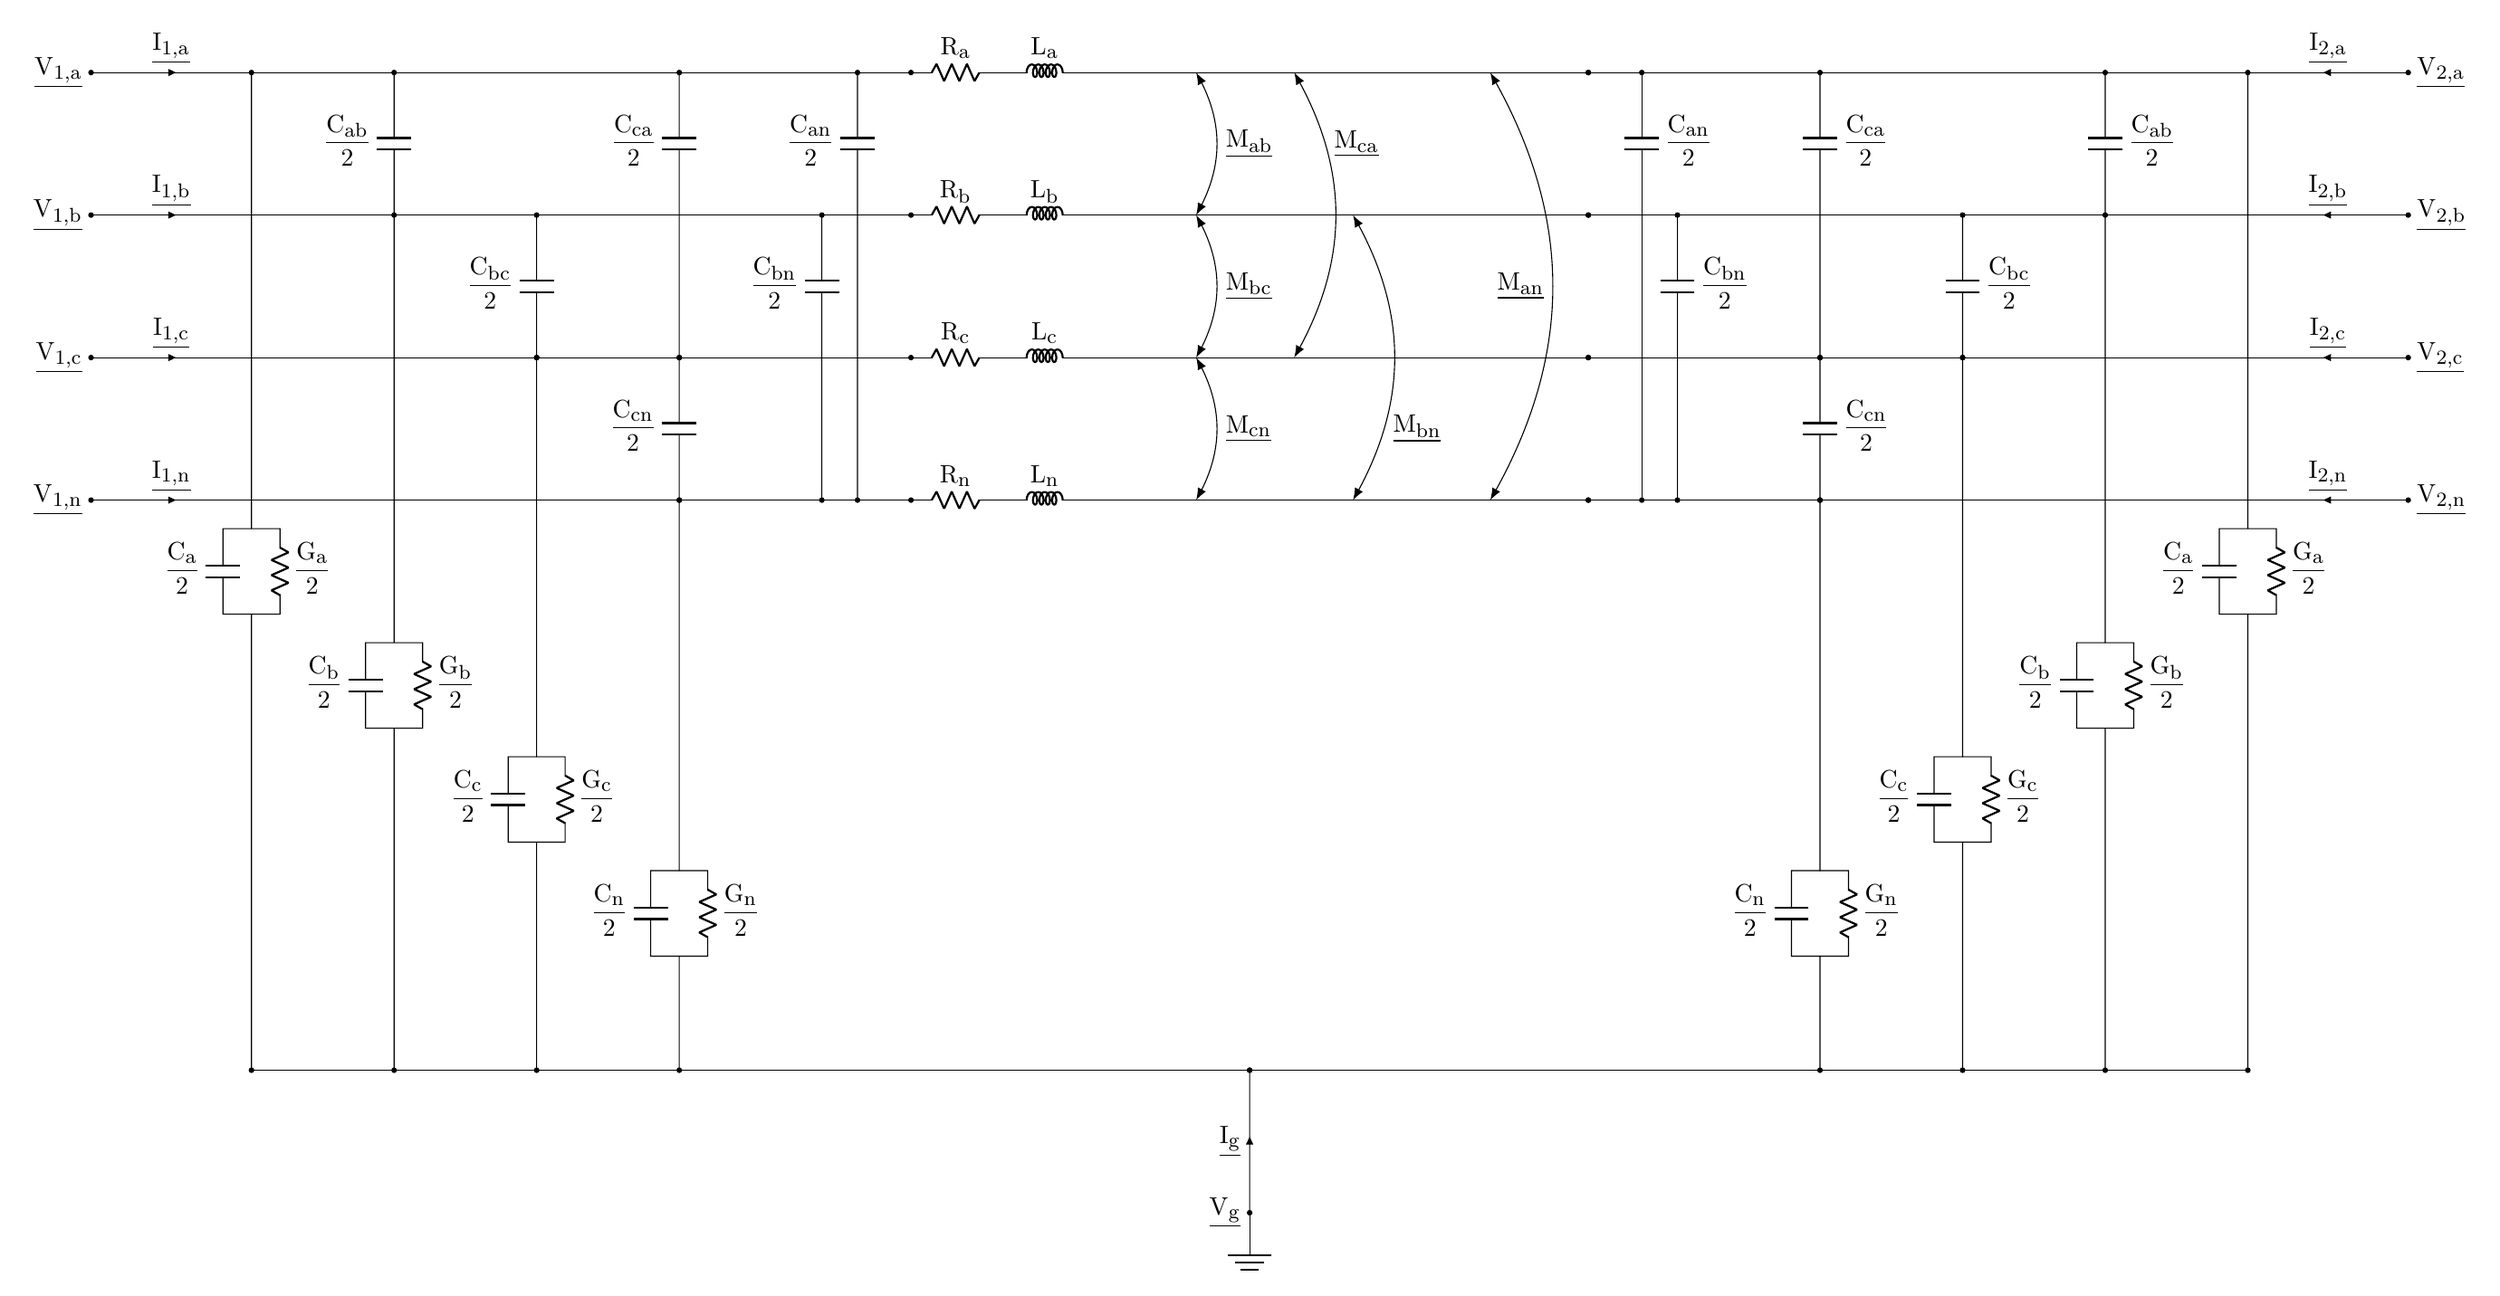
\begin{tikzpicture}[%
    show background rectangle,%
    tight background,%
    background rectangle/.style={fill=white}%
  ]
  % Version multifilaire

  %
  % Définitions
  %
  \pgfmathsetmacro{\xl}{0};%
  \pgfmathsetmacro{\zl}{11.5};%
  \pgfmathsetmacro{\xr}{\zl+2.5};%
  \pgfmathsetmacro{\xri}{\xr+1.5};%
  \pgfmathsetmacro{\zm}{21};%
  \pgfmathsetmacro{\xm}{32.5};%
  \pgfmathsetmacro{\xli}{2.25};%
  \pgfmathsetmacro{\xmi}{\xm-2.25};%
  \pgfmathsetmacro{\yt}{0};%
  \pgfmathsetmacro{\ytt}{-2};%
  \pgfmathsetmacro{\yn}{8};%
  \pgfmathsetmacro{\yc}{10};%
  \pgfmathsetmacro{\yb}{12};%
  \pgfmathsetmacro{\ya}{14};%

  %
  % Styles
  %
  \ctikzset{bipoles/length=0.8cm}%
  \tikzset{fleche/.style={<->,{Latex[]}-{Latex[]}}};%

  %
  % Coordonnées
  %
  \coordinate (orig) at (0,0);%

  % Début de ligne
  \coordinate (vlt) at (\xl,\yt);%
  \coordinate (vln) at (\xl,\yn);%
  \coordinate (vlc) at (\xl,\yc);%
  \coordinate (vlb) at (\xl,\yb);%
  \coordinate (vla) at (\xl,\ya);%

  % Fin de ligne
  \coordinate (vmt) at (\xm,\yt);%
  \coordinate (vmn) at (\xm,\yn);%
  \coordinate (vmc) at (\xm,\yc);%
  \coordinate (vmb) at (\xm,\yb);%
  \coordinate (vma) at (\xm,\ya);%

  % Début Z ligne
  \coordinate (zlt) at (\zl,\yt);%
  \coordinate (zln) at (\zl,\yn);%
  \coordinate (zlc) at (\zl,\yc);%
  \coordinate (zlb) at (\zl,\yb);%
  \coordinate (zla) at (\zl,\ya);%

  % Après résistance
  \coordinate (xrt) at (\xr,\yt);%
  \coordinate (xrn) at (\xr,\yn);%
  \coordinate (xrc) at (\xr,\yc);%
  \coordinate (xrb) at (\xr,\yb);%
  \coordinate (xra) at (\xr,\ya);%

  % Après résistance et courant
  \coordinate (xrit) at (\xri,\yt);%
  \coordinate (xrin) at (\xri,\yn);%
  \coordinate (xric) at (\xri,\yc);%
  \coordinate (xrib) at (\xri,\yb);%
  \coordinate (xria) at (\xri,\ya);%

  % Fin Z ligne
  \coordinate (zmt) at (\zm,\yt);%
  \coordinate (zmn) at (\zm,\yn);%
  \coordinate (zmc) at (\zm,\yc);%
  \coordinate (zmb) at (\zm,\yb);%
  \coordinate (zma) at (\zm,\ya);%

  % Première 1/2 admittance
  \coordinate (xlit) at (\xli,\yt);%
  \coordinate (xlin) at (\xli,\yn);%
  \coordinate (xlic) at (\xli,\yc);%
  \coordinate (xlib) at (\xli,\yb);%
  \coordinate (xlia) at (\xli,\ya);%

  % Seconde 1/2 admittance
  \coordinate (xmit) at (\xmi,\yt);%
  \coordinate (xmin) at (\xmi,\yn);%
  \coordinate (xmic) at (\xmi,\yc);%
  \coordinate (xmib) at (\xmi,\yb);%
  \coordinate (xmia) at (\xmi,\ya);%

  % Terre
  \coordinate (g) at (\zl/2+\zm/2,\yt);%
  \coordinate (g2) at (\zl/2+\zm/2,\ytt);%

  %
  % Dessin
  %
  % Tensions amont
  \node[left] at (vla) {$\underline{V_{1,\arm}}$};%
  \node[left] at (vlb) {$\underline{V_{1,\brm}}$};%
  \node[left] at (vlc) {$\underline{V_{1,\crm}}$};%
  \node[left] at (vln) {$\underline{V_{1,\nrm}}$};%

  % Tensions aval
  \node[right] at (vma) {$\underline{V_{2,\arm}}$};%
  \node[right] at (vmb) {$\underline{V_{2,\brm}}$};%
  \node[right] at (vmc) {$\underline{V_{2,\crm}}$};%
  \node[right] at (vmn) {$\underline{V_{2,\nrm}}$};%

  % Tension terre
  \node[ground, \circuitikzbasekey/bipoles/length=2cm] at (g2) {};%
  \node[left] at (g2) {$\underline{V_{\grm}}$};%

  % Câbles principaux
  % Terre
  \draw (xlit) to[short,-*] (g) to (xmit);%
  \draw (xlit) to[short,-*] (g) to (xmit);%
  \draw (g2) to[short, i=$\underline{I_{\grm}}$, *-] (g);%
  % Neutre
  \draw (vln) to[short,*-,i=$\underline{I_{1,\nrm}}$] (xlin) %
  to[short, -*] (zln)%
  to[R,l=$R_{\nrm}$] ($(zln)!0.5!(xrn)$)%
  to[L,l=$L_{\nrm}$] (xrn)%
  to[short,-] (xrin)%
  to[short,-*] (zmn)%
  to[short,*-] (xmin)%
  to[short,-*,i<=$\underline{I_{2,\nrm}}$] (vmn);%
  % C
  \draw (vlc) to[short,*-,i=$\underline{I_{1,\crm}}$] (xlic)%
  to[short, -*] (zlc)%
  to[R,l=$R_{\crm}$] ($(zlc)!0.5!(xrc)$)%
  to[L,l=$L_{\crm}$] (xrc)%
  to[short,-] (xric)%
  to[short,-*] (zmc)%
  to[short,*-] (xmic)%
  to[short,-*,i<=$\underline{I_{2,\crm}}$] (vmc);%
  % B
  \draw (vlb) to[short,*-,i=$\underline{I_{1,\brm}}$] (xlib)%
  to[short, -*] (zlb)%
  to[R,l=$R_{\brm}$] ($(zlb)!0.5!(xrb)$) %
  to[L,l=$L_{\brm}$] (xrb)%
  to[short,-] (xrib)%
  to[short,-*] (zmb)%
  to[short,*-] (xmib)%
  to[short,-*,i<=$\underline{I_{2,\brm}}$] (vmb);%
  % A
  \draw (vla) to[short,*-,i=$\underline{I_{1,\arm}}$] (xlia)%
  to[short, -*] (zla)%
  to[R,l=$R_{\arm}$] ($(zla)!0.5!(xra)$)%
  to[L,l=$L_{\arm}$] (xra)%
  to[short,-] (xria)%
  to[short,-*] (zma)%
  to[short,*-] (xmia)%
  to[short,-*,i<=$\underline{I_{2,\arm}}$] (vma);%

  % Mutuelles des lignes
  \pgfmathsetmacro{\xrm}{\xri+0.0*(\zm-\xri)};%
  \draw[fleche] (\xrm,\ya) to[bend left] node[midway, right]{$\underline{M_{\abrm}}$} (\xrm,\yb);%
  \draw[fleche] (\xrm,\yb) to[bend left] node[midway, right]{$\underline{M_{\bcrm}}$} (\xrm,\yc);%
  \draw[fleche] (\xrm,\yc) to[bend left] node[midway, right]{$\underline{M_{\cnrm}}$} (\xrm,\yn);%
  \pgfmathsetmacro{\xrm}{\xri+0.25*(\zm-\xri)};%
  \draw[fleche] (\xrm,\ya) to[bend left] node[near start, right]{$\underline{M_{\carm}}$} (\xrm,\yc);%
  \pgfmathsetmacro{\xrm}{\xri+0.40*(\zm-\xri)};%
  \draw[fleche] (\xrm,\yb) to[bend left] node[near end, right]{$\underline{M_{\bnrm}}$} (\xrm,\yn);%
  \pgfmathsetmacro{\xrm}{\xri+0.75*(\zm-\xri)};%
  \draw[fleche] (\xrm,\ya) to[bend left] node[midway, left]{$\underline{M_{\anrm}}$} (\xrm,\yn);%

  % Première 1/2 admittance
  \pgfmathsetmacro{\ylihaut}{\yt+0.95*(\yn-\yt)};%
  \pgfmathsetmacro{\ylibas}{\ylihaut-1.2};%
  \pgfmathsetmacro{\xliplus}{\xli+0.4};%
  \pgfmathsetmacro{\xlimoins}{\xli-0.4};%
  \draw (xlia) to[short,*-] (\xli,\ylihaut) -| (\xliplus,\ylihaut)%
  to[R=$\dfrac{G_{\arm}}{2}$] (\xliplus,\ylibas) |- (\xli,\ylibas)%
  to[short,-*] (\xli,\yt);%
  \draw (\xli,\ylihaut) -| (\xlimoins,\ylihaut) to[C,l_=$\dfrac{C_{\arm}}{2}$] (\xlimoins,\ylibas) |- (\xli,\ylibas);%

  \pgfmathsetmacro{\ylihaut}{\yt+0.75*(\yn-\yt)};%
  \pgfmathsetmacro{\ylibas}{\ylihaut-1.2};%
  \pgfmathsetmacro{\xliref}{\xli+2};%
  \pgfmathsetmacro{\xliplus}{\xliref+0.4};%
  \pgfmathsetmacro{\xlimoins}{\xliref-0.4};%
  \coordinate (ref) at (\xliref,0);%
  \draw (xlib -| ref) to[short,*-] (\xliref,\ylihaut) -| (\xliplus,\ylihaut)%
  to[R=$\dfrac{G_{\brm}}{2}$] (\xliplus,\ylibas) |- (\xliref,\ylibas)%
  to[short,-*] (\xliref,\yt);%
  \draw (\xliref,\ylihaut) -| (\xlimoins,\ylihaut)%
  to[C,l_=$\dfrac{C_{\brm}}{2}$] (\xlimoins,\ylibas) |- (\xliref,\ylibas);%
  \draw (xlia -| ref) to[C,l_=$\dfrac{C_{\abrm}}{2}$,*-] (xlib -|  ref);%

  \pgfmathsetmacro{\ylihaut}{\yt+0.55*(\yn-\yt)};%
  \pgfmathsetmacro{\ylibas}{\ylihaut-1.2};%
  \pgfmathsetmacro{\xliref}{\xli+4}
  \pgfmathsetmacro{\xliplus}{\xliref+0.4};%
  \pgfmathsetmacro{\xlimoins}{\xliref-0.4};%
  \coordinate (ref) at (\xliref,0);%
  \draw (xlic -| ref) to[short,*-] (\xliref,\ylihaut) -| (\xliplus,\ylihaut)%
  to[R=$\dfrac{G_{\crm}}{2}$] (\xliplus,\ylibas) |- (\xliref,\ylibas)%
  to[short,-*] (\xliref,\yt);%
  \draw (\xliref,\ylihaut) -| (\xlimoins,\ylihaut) %
  to[C,l_=$\dfrac{C_{\crm}}{2}$] (\xlimoins,\ylibas) |- (\xliref,\ylibas);%
  \draw (xlib -| ref) to[C,l_=$\dfrac{C_{\bcrm}}{2}$,*-*] (xlic -| ref);%

  \pgfmathsetmacro{\ylihaut}{\yt+0.35*(\yn-\yt)};%
  \pgfmathsetmacro{\ylibas}{\ylihaut-1.2};%
  \pgfmathsetmacro{\xliref}{\xli+6}
  \pgfmathsetmacro{\xliplus}{\xliref+0.4};%
  \pgfmathsetmacro{\xlimoins}{\xliref-0.4};%
  \coordinate (ref) at (\xliref,0);%
  \draw (xlin -| ref) to[short,*-] (\xliref,\ylihaut) -| (\xliplus,\ylihaut)%
  to[R=$\dfrac{G_{\nrm}}{2}$] (\xliplus,\ylibas) |- (\xliref,\ylibas)%
  to[short,-*] (\xliref,\yt);%
  \draw (\xliref,\ylihaut) -| (\xlimoins,\ylihaut)%
  to[C,l_=$\dfrac{C_{\nrm}}{2}$] (\xlimoins,\ylibas) |- (\xliref,\ylibas);%
  \draw (xlic -| ref) to[C,l_=$\dfrac{C_{\cnrm}}{2}$,*-*] (xlin -| ref);%
  \draw (xlia -| ref) to[C,l_=$\dfrac{C_{\carm}}{2}$,*-] (xlib -| ref) to[short,-*] (xlic -| ref);%

  \pgfmathsetmacro{\xliref}{\xli+8};%
  \coordinate (ref) at (\xliref,0);%
  \draw (xlib -| ref) to[C,l_=$\dfrac{C_{\bnrm}}{2}$,*-] (xlic -| ref) to[short,-*] (xlin -| ref);%
  \pgfmathsetmacro{\xliref}{\xli+8.5};%
  \coordinate (ref) at (\xliref,0);%
  \draw (xlia -| ref) to[C,l_=$\dfrac{C_{\anrm}}{2}$,*-] (xlib -| ref) to[short,-*] (xlin -| ref);%

  % Seconde 1/2 admittance
  \pgfmathsetmacro{\ymihaut}{\yt+0.95*(\yn-\yt)};%
  \pgfmathsetmacro{\ymibas}{\ymihaut-1.2};%
  \pgfmathsetmacro{\xmiplus}{\xmi+0.4};%
  \pgfmathsetmacro{\xmimoins}{\xmi-0.4};%
  \draw (xmia) to[short,*-] (\xmi,\ymihaut) -| (\xmiplus,\ymihaut) %
  to[R,l=$\dfrac{G_{\arm}}{2}$] (\xmiplus,\ymibas) |- (\xmi,\ymibas) %
  to[short,-*] (\xmi,\yt);%
  \draw (\xmi,\ymihaut) -| (\xmimoins,\ymihaut) to[C,l_=$\dfrac{C_{\arm}}{2}$] (\xmimoins,\ymibas) |- (\xmi,\ymibas);%

  \pgfmathsetmacro{\ymihaut}{\yt+0.75*(\yn-\yt)};%
  \pgfmathsetmacro{\ymibas}{\ymihaut-1.2};%
  \pgfmathsetmacro{\xmiref}{\xmi-2};%
  \pgfmathsetmacro{\xmiplus}{\xmiref+0.4};%
  \pgfmathsetmacro{\xmimoins}{\xmiref-0.4};%
  \coordinate (ref) at (\xmiref,0);%
  \draw (xmib -| ref) to[short,*-] (\xmiref,\ymihaut) -| (\xmiplus,\ymihaut)%
  to[R,l=$\dfrac{G_{\brm}}{2}$] (\xmiplus,\ymibas) |- (\xmiref,\ymibas)%
  to[short,-*] (\xmiref,\yt);%
  \draw (\xmiref,\ymihaut) -| (\xmimoins,\ymihaut)%
  to[C,l_=$\dfrac{C_{\brm}}{2}$] (\xmimoins,\ymibas) |- (\xmiref,\ymibas);%
  \draw (xmia -| ref) to[C,l^=$\dfrac{C_{\abrm}}{2}$,*-] (xmib -| ref);%

  \pgfmathsetmacro{\ymihaut}{\yt+0.55*(\yn-\yt)};%
  \pgfmathsetmacro{\ymibas}{\ymihaut-1.2};%
  \pgfmathsetmacro{\xmiref}{\xmi-4}
  \pgfmathsetmacro{\xmiplus}{\xmiref+0.4};%
  \pgfmathsetmacro{\xmimoins}{\xmiref-0.4};%
  \coordinate (ref) at (\xmiref,0);%
  \draw (xmic -| ref) to[short,*-] (\xmiref,\ymihaut) -| (\xmiplus,\ymihaut)%
  to[R,l=$\dfrac{G_{\crm}}{2}$] (\xmiplus,\ymibas) |- (\xmiref,\ymibas)%
  to[short,-*] (\xmiref,\yt);%
  \draw (\xmiref,\ymihaut) -| (\xmimoins,\ymihaut)%
  to[C,l_=$\dfrac{C_{\crm}}{2}$] (\xmimoins,\ymibas) |- (\xmiref,\ymibas);%
  \draw (xmib -| ref) to[C,l^=$\dfrac{C_{\bcrm}}{2}$,*-*] (xmic -| ref);%

  \pgfmathsetmacro{\ymihaut}{\yt+0.35*(\yn-\yt)};%
  \pgfmathsetmacro{\ymibas}{\ymihaut-1.2};%
  \pgfmathsetmacro{\xmiref}{\xmi-6}
  \pgfmathsetmacro{\xmiplus}{\xmiref+0.4};%
  \pgfmathsetmacro{\xmimoins}{\xmiref-0.4};%
  \coordinate (ref) at (\xmiref,0);%
  \draw (xmin -| ref) to[short,*-] (\xmiref,\ymihaut) -| (\xmiplus,\ymihaut)%
  to[R,l=$\dfrac{G_{\nrm}}{2}$] (\xmiplus,\ymibas) |- (\xmiref,\ymibas)%
  to[short,-*] (\xmiref,\yt);%
  \draw (\xmiref,\ymihaut) -| (\xmimoins,\ymihaut)%
  to[C,l_=$\dfrac{C_{\nrm}}{2}$] (\xmimoins,\ymibas) |- (\xmiref,\ymibas);%
  \draw (xmic -| ref) to[C,l^=$\dfrac{C_{\cnrm}}{2}$,*-*] (xmin -| ref);%
  \draw (xmia -| ref) to[C,l^=$\dfrac{C_{\carm}}{2}$,*-] (xmib -| ref) to[short,-*] (xmic -| ref);%

  \pgfmathsetmacro{\xmiref}{\xmi-8};%
  \coordinate (ref) at (\xmiref,0);%
  \draw (xmib -| ref) to[C,l^=$\dfrac{C_{\bnrm}}{2}$,*-] (xmic -| ref) to[short,-*] (xmin -| ref);%
  \pgfmathsetmacro{\xmiref}{\xmi-8.5};%
  \coordinate (ref) at (\xmiref,0);%
  \draw (xmia -| ref) to[C,l^=$\dfrac{C_{\anrm}}{2}$,*-] (xmib -| ref) to[short,-*] (xmin -| ref);%
\end{tikzpicture}
\end{document}
% Local Variables:
% mode: latex
% TeX-engine: luatex
% TeX-source-correlate-method-active: synctex
% ispell-local-dictionary: "british"
% coding: utf-8
% LaTeX-indent-level: 2
% fill-column: 120
% End:
